\chapter{Semiconductor Bandstructure}

\section{Introduction}
The behavior of electrons in semiconductors is governed by the solutions to the Schrödinger equation tailored to the crystal environment. These solutions yield the electronic bandstructure, which characterizes the allowed energy states for electrons in the material. Determining the electronic spectrum is, however, a highly complex task. In solids, the presence of a vast number of atoms arranged closely together generates a complicated potential energy landscape for electrons. Furthermore, electron–electron interactions and dynamic lattice vibrations (phonons) introduce additional complexity through time-dependent variations in the potential.
To make the problem tractable, the effects of atomic vibrations and electron–electron scattering are initially excluded and later incorporated using perturbation theory. These effects primarily contribute to the scattering of electrons between different quantum states.
The analysis of bandstructure becomes significantly more manageable in crystalline solids. In such systems, the electrons move in a spatially periodic potential due to the regular arrangement of atoms. This periodicity leads to solutions that obey Bloch’s theorem, which will be addressed in the following section.
Realistic methods for computing the bandstructure of semiconductors generally fall into two broad categories:
\begin{enumerate}
	\item Approaches that capture the full conduction and valence band profiles.
	\item Approaches that focus specifically on the bandstructure near the band edges.
\end{enumerate}

\section{Block Theorem and Crystal Momentum}
To analyze the electronic characteristics of a material, it is essential to determine the electron wavefunctions and their corresponding energies within a solid. In this context, we focus solely on crystalline materials. The behavior of electrons in a periodic solid is governed by the Schrödinger equation:

\begin{equation*}
	\left[-\frac{\hbar^2}{2m} \nabla^2 + U(\mathbf{r})\right] \psi(\mathbf{r}) = E \psi(\mathbf{r})
\end{equation*}

Here, \( U(\mathbf{r}) \) represents the potential energy experienced by the electrons. Owing to the periodic structure of the crystal, this potential exhibits the same periodicity \( \mathbf{R} \) as the lattice:

\begin{equation*}
	U(\mathbf{r}) = U(\mathbf{r} + \mathbf{R})
\end{equation*}

In the case where the background potential is absent, the electron wavefunction within a volume \( V \) takes the form \( \psi(\mathbf{r}) = \frac{1}{\sqrt{V}} e^{i\mathbf{k} \cdot \mathbf{r}} \), and the corresponding momentum and energy of the electron are given by:

\begin{equation*}
	\mathbf{p} = \hbar \mathbf{k}, \quad E = \frac{\hbar^2 k^2}{2m}
\end{equation*}

This wavefunction is delocalized over the entire sample, implying that the probability density \( \psi^* \psi \) is uniform throughout space.

When considering a periodic crystal, it is expected that the electron probability distribution remains identical in each unit cell, since all cells are structurally the same. If the potential were disordered, this uniformity would not hold. Given a lattice translation vector \( \mathbf{R} \), we require:

\begin{equation*}
	|\psi(\mathbf{r})|^2 = |\psi(\mathbf{r} + \mathbf{R})|^2
\end{equation*}

This condition ensures that one cannot distinguish between different unit cells based on electronic probability density. It is important to note that while the probability is periodic, the wavefunction itself need not be. The appropriate form of the wavefunction in a periodic potential is described by Bloch’s theorem. According to this theorem, the eigenfunctions of the Schrödinger equation in a periodic lattice are of the form:

\begin{equation*}
	\psi_{\mathbf{k}}(\mathbf{r}) = u_{\mathbf{k}}(\mathbf{r}) e^{i\mathbf{k} \cdot \mathbf{r}}
\end{equation*}

where \( u_{\mathbf{k}}(\mathbf{r}) \) is a function that shares the periodicity of the crystal:

\begin{equation*}
	u_{\mathbf{k}}(\mathbf{r}) = u_{\mathbf{k}}(\mathbf{r} + \mathbf{R})
\end{equation*}

\begin{center}
	\begin{minipage}{0.6\textwidth}
		\centering
		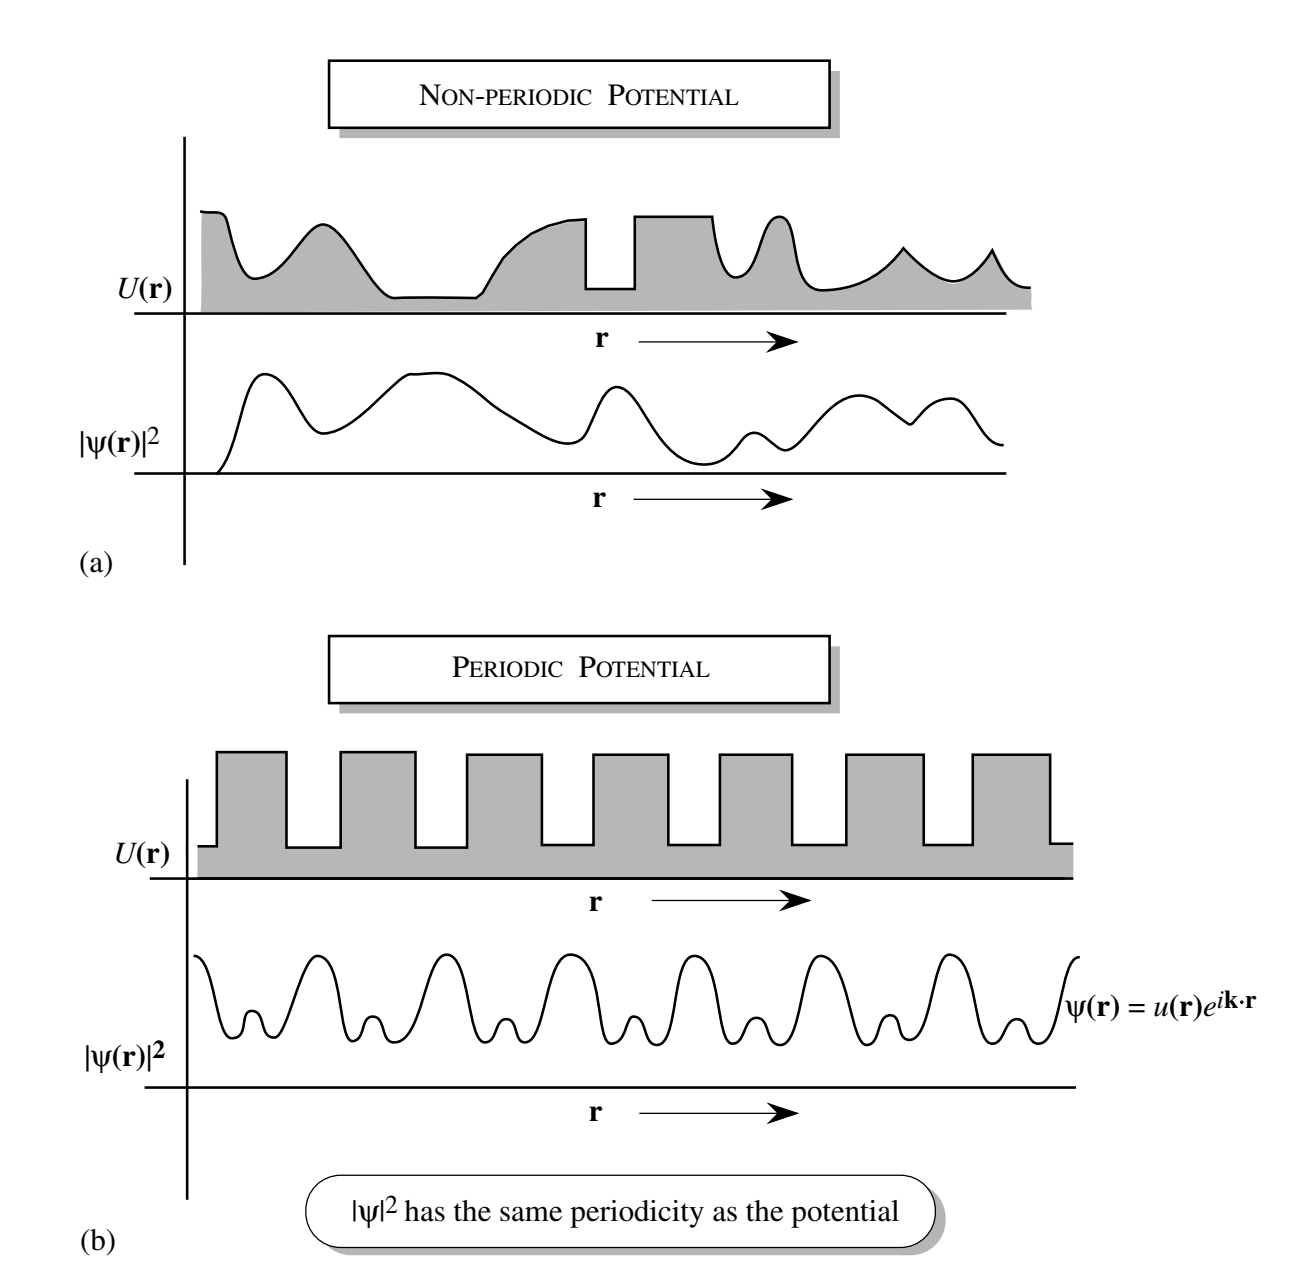
\includegraphics[width=\textwidth]{img/periodic_potential.png}
		\\[0.5em]
		\refstepcounter{figure}
		\textbf{Figure~\thefigure.} (a) Example of an electronic wavefunction in a disordered material. (b) In a periodic potential, \( |\psi|^2 \) shares the same periodicity, as required by Bloch's theorem.
		\label{fig:periodic_potential}
	\end{minipage}
\end{center}

This implies that the full wavefunction transforms under lattice translations as:

\begin{equation*}
	\psi_{\mathbf{k}}(\mathbf{r} + \mathbf{R}) = u_{\mathbf{k}}(\mathbf{r} + \mathbf{R}) e^{i\mathbf{k} \cdot (\mathbf{r} + \mathbf{R})} = u_{\mathbf{k}}(\mathbf{r}) e^{i\mathbf{k} \cdot \mathbf{r}} e^{i\mathbf{k} \cdot \mathbf{R}} = \psi_{\mathbf{k}}(\mathbf{r}) e^{i\mathbf{k} \cdot \mathbf{R}}
\end{equation*}
The vector \( \mathbf{k} \), known as the wavevector or \( \mathbf{k} \)-vector, is fundamental in describing the electronic properties of crystalline solids.

\subsection{Significance of the k-Vector}
One of the key consequences of Bloch's theorem is that, in a perfectly periodic potential provided by the crystal lattice, electrons can propagate through the material without experiencing scattering. In such a scenario, the electron wavefunction, which resembles \( \sim e^{i\mathbf{k} \cdot \mathbf{r}} \), describes an extended state that spans the entire crystal.
To understand how electrons behave under external influences, we seek to derive an equation of motion that captures their response to external forces. Let \( \mathbf{F}_{\text{ext}} \) denote an external force acting on the electron, and \( \mathbf{F}_{\text{int}} \) represent the internal force arising from the atomic lattice. Newton’s second law can then be expressed as:

\begin{equation*}
	\frac{d\mathbf{p}}{dt} = \mathbf{F}_{\text{ext}} + \mathbf{F}_{\text{int}}
\end{equation*}

\noindent However, this form is not particularly useful, as it involves the internal forces, which are typically complex to evaluate. To describe the electron's motion more effectively, we need an equation that depends solely on the external forces. We now outline a simplified derivation of such an expression, which also helps clarify the physical interpretation of the wavevector \( \mathbf{k} \) introduced in Bloch’s theorem.
Starting from the time-dependent Schrödinger equation, the general solution for electrons in a periodic potential can be written as:
\begin{equation*}
	\psi(\mathbf{r}, t) = u_{\mathbf{k}}(\mathbf{r}) e^{i(\mathbf{k} \cdot \mathbf{r} - \omega t)}
\end{equation*}

\noindent where the energy of the electron is connected to the angular frequency \( \omega \) by the relation:

\begin{equation*}
	E = \hbar \omega
\end{equation*}

\noindent The Bloch function thus corresponds to a plane wave that extends throughout the crystalline solid. To describe a spatially localized electron, we consider a wavepacket composed of Bloch states centered around a specific wavevector \( \mathbf{k} \). The group velocity of this wavepacket is given by:

\begin{equation*}
	\mathbf{v}_g = \frac{d\omega}{d\mathbf{k}} = \frac{1}{\hbar} \frac{dE}{d\mathbf{k}} = \frac{1}{\hbar} \nabla_{\mathbf{k}} E(\mathbf{k})
\end{equation*}

In the presence of an electric field \( \mathbf{F} \), the energy gained by the electron over a short time interval \( \delta t \) is:

\begin{equation*}
	\delta E = -e \mathbf{F} \cdot \mathbf{v}_g \, \delta t
\end{equation*}

\noindent More generally, the change in energy can be expressed as:

\begin{equation*}
	\delta E = \frac{dE}{d\mathbf{k}} \cdot \delta \mathbf{k} = \hbar \mathbf{v}_g \cdot \delta \mathbf{k}
\end{equation*}

\noindent Equating the two expressions for \( \delta E \), we obtain:

\begin{equation*}
	\delta \mathbf{k} = -\frac{e \mathbf{F}}{\hbar} \delta t
\end{equation*}

\noindent which leads to the equation of motion for the wavevector:

\begin{equation*}
	\hbar \frac{d\mathbf{k}}{dt} = -e \mathbf{F}
\end{equation*}

\noindent Since \( -e\mathbf{F} \) is the force acting on the electron, this can be generalized to:

\begin{equation*}
	\hbar \frac{d\mathbf{k}}{dt} = \mathbf{F}_{\text{ext}}
\end{equation*}

\noindent This result mirrors Newton’s second law:

\begin{equation*}
	\frac{d\mathbf{p}}{dt} = \mathbf{F}_{\text{ext}}
\end{equation*}

\noindent provided we identify \( \hbar d\mathbf{k} \) with the momentum of the electron inside the crystal. While \( \hbar d\mathbf{k} \) behaves as the momentum in response to external forces, it is not the true mechanical momentum since it incorporates the effects of the internal periodic potential. Instead, \( \hbar \mathbf{k} \) is referred to as the \textit{crystal momentum}.

\section{Metals, Insulators, and Semiconductors}
From atomic physics, it is known that bound electrons occupy discrete energy levels, separated by regions where no states exist. In solids, these discrete levels broaden into continuous energy bands, with forbidden gaps—bandgaps—separating them. Once the electronic band structure is known, a key question arises: which of the available states are occupied by electrons, and which remain empty?
Two important cases emerge regarding electron occupation: in one scenario, an energy band is fully occupied at 0~K, while the next higher band is separated by an energy gap \( E_g \) and remains completely unoccupied. In the second case, the highest energy band that contains electrons is only partially filled.
At this stage, a critical concept must be introduced. When an energy band is completely filled, the electrons within it cannot contribute to electrical conduction. This is a direct consequence of the Pauli exclusion principle: since electrons are fermions, they can only transition into unoccupied states. In a filled band, all such states are already occupied, leading to a cancellation of net motion—electrons moving in opposite directions balance each other. As a result, materials with fully filled bands and an energy gap above them exhibit, in principle, infinite resistivity and are classified as insulators or semiconductors.
In contrast, if the highest occupied band is only partially filled, available empty states exist within the same band. This allows electrons to accelerate under an external field, enabling electrical conduction. Such materials exhibit low resistivity and are termed metals.
\begin{center}
	\begin{minipage}{0.6\textwidth}
		\centering
		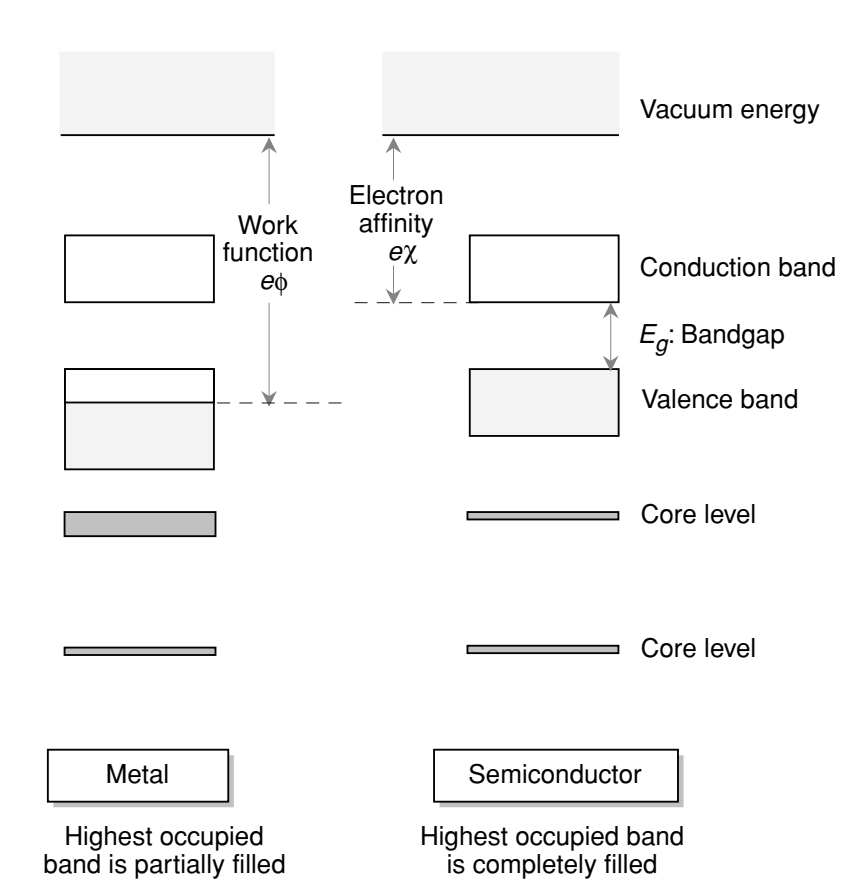
\includegraphics[width=\textwidth]{img/metalsVSsemiconductors.png}
		\\[0.5em]
		\refstepcounter{figure}
		\textbf{Figure~\thefigure.} Band occupation at 0~K for a metal and a semiconductor. In metals, the top band is partially filled. In semiconductors, the valence band is full and separated from the empty conduction band by the bandgap \( E_g \). Work function and electron affinity are indicated.
		\label{fig:metalsVSsemiconductors}
	\end{minipage}
\end{center}
The band that is fully occupied by electrons at absolute zero in semiconductors is known as the \textit{valence band}, whereas the higher energy band that remains empty at 0~K is referred to as the \textit{conduction band}. In metals, the energy difference between the vacuum level and the highest occupied electronic state is termed the \textit{work function}. For semiconductors, the energy separating the vacuum level from the bottom of the conduction band is called the \textit{electron affinity}.
Metals are characterized by extremely high electrical conductivity, resulting from the large number of electrons available for conduction. However, this abundance of charge carriers also makes it difficult to significantly modify their conductivity. Semiconductors, in contrast, exhibit zero conductivity at 0~K and relatively low conductivity at finite temperatures. Importantly, their conductivity can be altered dramatically—by several orders of magnitude—which is the foundation of their utility in active electronic components.
As previously discussed, semiconductors are defined as materials in which the valence band is completely filled and the conduction band completely empty at 0~K. When the temperature is raised above absolute zero, some electrons gain enough thermal energy to transition from the valence band into the conduction band. This results in the creation of empty states (holes) in the valence band and free electrons in the conduction band.
